\chapter{Techniques de laboratoire III~: la pratique de la recherche}\label{ch:b3:lab-techniques-3}

Un flacon de solution de butyllithium prend feu si une goutte rencontre
l'air~; une \omterm{def:b3:lab-techniques-3:schlenk}{boîte à gants} maintient le dioxygène et l'eau au-dessous de
quelques parties par million pour qu'on puisse peser de tels composés
comme du sel de table. La chimie de recherche commence souvent par tenir
l'atmosphère à l'écart, et finit par une affirmation que d'autres doivent
pouvoir vérifier~: un nouveau composé, sa structure et sa pureté prouvées
par plusieurs méthodes indépendantes, ses données consignées et publiées
pour que le travail puisse être reproduit. Ce dernier chapitre rassemble
la pratique de la recherche~: manipuler des substances sensibles à l'air,
caractériser un nouveau composé, juger statistiquement un résultat, tenir
un \omterm{def:b3:lab-techniques-3:notebook}{cahier de laboratoire} et lire la littérature, et évaluer les risques
d'un mode opératoire que personne n'a encore mis en œuvre.

\begin{recall}
Le volume de première année a traité des dangers, des risques, des
pictogrammes, des mentions H et P, des fiches de données de sécurité et de
l'incertitude de mesure avec ses évaluations de type A et B~; le volume de
deuxième année, des atmosphères inertes, du traitement, des desséchants, de
la chromatographie éclair, de la spectrométrie de masse (HRMS, masse
monoisotopique), de la RMN du $^{13}$C, des intervalles de confiance,
du coefficient de Student, de l'étalonnage, de la fidélité, de la justesse,
du biais, de la répétabilité, de la validation de méthode, de l'élévation
adiabatique de température et de l'emballement thermique. Le
\cref{ch:b3:advanced-nmr}, le \cref{ch:b3:x-ray-diffraction} et le
\cref{ch:b3:electrode-kinetics} ont fourni les méthodes structurales et
électrochimiques.
\end{recall}

\begin{omfigure}
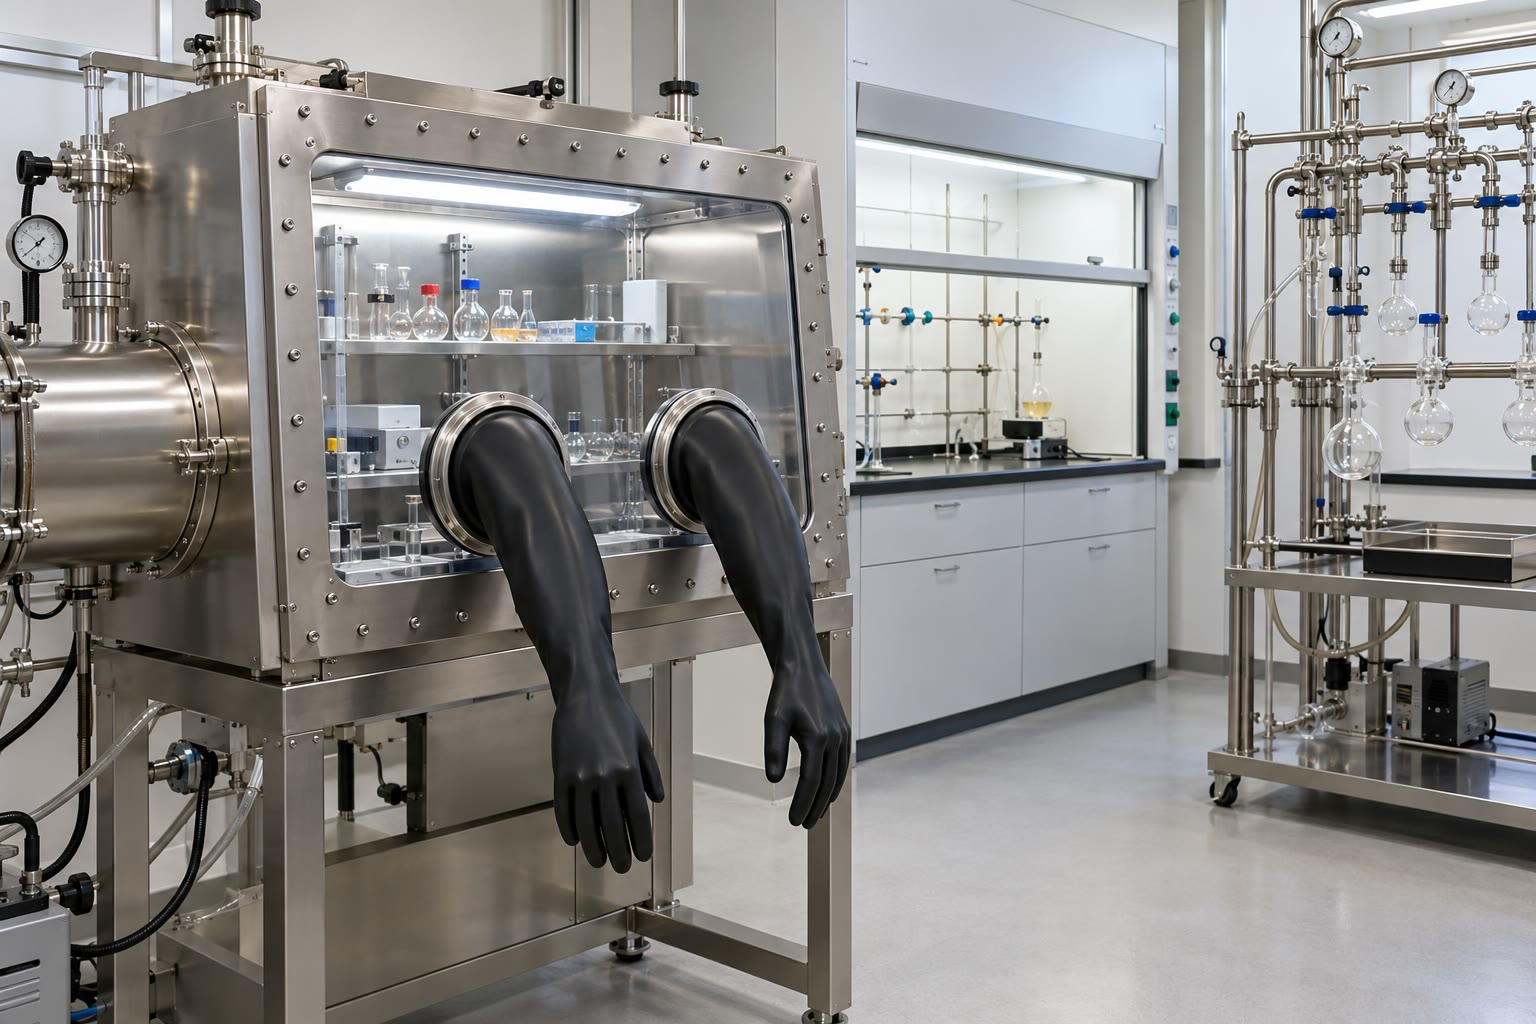
\includegraphics[width=0.58\linewidth]{images/book4/ai/b3-33-glovebox.jpg}

{\small Un laboratoire de recherche équipé d'une \omterm{def:b3:lab-techniques-3:schlenk}{boîte à gants}~: on
travaille dans le caisson en acier inoxydable, rempli de diazote ou
d'argon sec, à travers les gants~; le cylindre à gauche est le sas qui
permet d'entrer et de sortir les objets.}
\end{omfigure}

\section{Travailler sans air}

\begin{definition}[Composés sensibles à l'air]\label{def:b3:lab-techniques-3:air-sensitive}
Un \emph{composé sensible à l'air}\index{compose sensible a l'air@composé sensible à l'air} réagit avec le
dioxygène ou l'eau de l'air, en se décomposant ou en perdant son activité.
Une \emph{substance pyrophorique}\index{substance pyrophorique} s'enflamme
spontanément à l'air.
\end{definition}

\begin{definition}[Rampe de Schlenk et boîte à gants]\label{def:b3:lab-techniques-3:schlenk}
Une \emph{rampe de Schlenk}\index{rampe de Schlenk} est une double rampe
en verre, dont un tube est relié à une pompe à vide par l'intermédiaire
d'un piège froid et l'autre à une alimentation en gaz inerte sec qui
s'échappe par un bulleur à huile, avec des robinets qui relient chaque
sortie à l'un ou à l'autre. Un \emph{tube de Schlenk}\index{tube de Schlenk} possède un bras
latéral muni d'un robinet pour le raccorder à la rampe. Une \emph{boîte à gants}\index{boite a gants@boîte à gants} est une enceinte
étanche remplie de gaz inerte, purifié en continu, dans laquelle on
travaille à travers des gants.
\end{definition}

\begin{omfigure}
\begin{tikzpicture}[font=\scriptsize, >=Stealth]
  % manifolds
  \draw[om glass, line width=1.1pt] (0,3.0) -- (8.0,3.0);
  \draw[om glass, line width=1.1pt] (0,2.5) -- (8.0,2.5);
  \node[anchor=east] at (-1.0,3.0) {gaz inerte};
  \node[anchor=east] at (0,2.5) {vide};
  % taps
  \foreach \x in {2.0,4.0,6.0} {
    \draw[om glass] (\x,3.0) -- (\x,2.5);
    \draw[fill=white] (\x,2.75) circle (0.12);
    \draw (\x-0.1,2.75) -- (\x+0.1,2.75);
    \draw[om glass] (\x,2.5) -- (\x,2.0);
  }
  % flask on the middle tap
  \draw[thick, black!60] (4.0,2.0) -- (4.0,1.6) -- (4.6,1.6);
  \pic[scale=0.5, transform shape] at (5.0,-0.2) {rbflask={0.3}{omDef!20}};
  \draw[om glass] (4.6,1.6) -- (4.9,1.25);
  \node[anchor=west] at (5.4,0.4) {tube de Schlenk};
  % bubbler at the gas end
  \pic[scale=0.55, transform shape] at (8.9,1.5) {bubbler};
  \draw[om glass] (8.0,3.0) -- (8.6,3.0) -- (8.6,2.9);
  \node[anchor=west] at (9.4,2.2) {bulleur à huile};
  % trap and pump at the vacuum end
  \draw[om glass] (0.4,2.5) -- (0.4,1.6);
  \draw[om glass, fill=omDef!8] (0.15,1.6) rectangle (0.65,0.4);
  \fill[omDef!25] (0.0,0.2) rectangle (0.8,1.2);
  \node[anchor=north] at (0.4,0.2) {piège froid};
  \draw[om glass] (0.65,0.9) -- (1.6,0.9);
  \draw[fill=black!15] (1.6,0.6) rectangle (2.6,1.2);
  \node at (2.1,0.9) {pompe};
  \draw[->, thick] (-0.9,3.0) -- (0,3.0);
\end{tikzpicture}

{\small Une \omterm{def:b3:lab-techniques-3:schlenk}{rampe de Schlenk}, schématique~: une rampe de gaz et une rampe de
vide reliées par des robinets~; chaque robinet relie son tube soit au
vide, soit au gaz inerte. Les vapeurs de solvant pompées se condensent dans
le piège froid avant d'atteindre la pompe~; le gaz s'échappe par un
bulleur à huile, qui empêche l'air de refluer.}
\end{omfigure}

\begin{proposition}[Cycles vide--remplissage]\label{prop:b3:lab-techniques-3:purge-cycles}
Si un récipient rempli d'air à la pression $p_0$ est vidé jusqu'à $p_{\min}$ puis rempli de
gaz inerte pur, $n$ fois, la fraction de l'air initial qui reste vaut $(p_{\min}/p_0)^n$.
\end{proposition}

\begin{proof}
Le pompage jusqu'à $p_{\min}$ laisse une fraction $p_{\min}/p_0$ du gaz, de même composition~; le
remplissage par du gaz inerte pur rétablit $p_0$ sans ajouter d'air. Chaque cycle multiplie la
fraction d'air par $p_{\min}/p_0$~; après $n$ cycles, $(p_{\min}/p_0)^n$.
\end{proof}

Trois cycles à \qty{0.1}{mbar} laissent sur le papier $10^{-12}$ de l'air~; en pratique, les fuites, le gaz
adsorbé sur le verre et le dégazage de la graisse et des septums fixent la
limite, ce qui explique que la verrerie soit séchée à l'étuve et assemblée
à chaud.

\begin{definition}[Transfert par canule]\label{def:b3:lab-techniques-3:cannula}
Un \emph{transfert par canule}\index{transfert par canule} fait passer un
liquide sensible à l'air d'un récipient fermé à un autre par une longue
aiguille à deux pointes, sous l'effet d'une légère surpression de gaz
inerte dans le premier récipient.
\end{definition}

\begin{omfigure}
\begin{tikzpicture}[font=\scriptsize, >=Stealth]
  \pic at (0,0) {rbflask={0.35}{omThm!25}};
  \pic at (4.2,0) {rbflask={0.1}{omDef!15}};
  \pic at (0,3.0) {septum};
  \pic at (4.2,3.0) {septum};
  \draw[black!70, line width=0.9pt] (0.05,0.25) -- (0.05,3.5) to[out=90, in=90] (4.15,3.5) -- (4.15,1.6);
  \draw[->, thick, omThm] (1.3,3.95) -- (2.9,3.95) node[midway, above] {liquide};
  \draw[->, thick] (-1.3,3.4) -- (-0.15,3.2) node[pos=0, left] {arrivée de gaz inerte (légère surpression)};
  \draw[->, thick] (4.35,3.2) -- (5.4,3.6) node[right] {sortie vers le bulleur};
  \node[anchor=north] at (0,-0.1) {source};
  \node[anchor=north] at (4.2,-0.1) {récepteur};
\end{tikzpicture}

{\small Un \omterm{def:b3:lab-techniques-3:cannula}{transfert par canule}~: l'extrémité inférieure de la canule plonge
dans le liquide du ballon source~; le gaz inerte admis dans la source
pousse le liquide à travers la canule jusqu'au récepteur, mis à l'air par
une aiguille reliée au bulleur.}
\end{omfigure}

\begin{method}[Un transfert par canule]\label{met:b3:lab-techniques-3:cannula}
\begin{enumerate}
  \item Placer les deux ballons, fermés par des septums, sous gaz inerte
        sur la \omterm{def:b3:lab-techniques-3:schlenk}{rampe de Schlenk}.
  \item Purger la canule avec le gaz~: introduire une extrémité dans la
        source au-dessus du liquide jusqu'à ce que le gaz sorte par l'autre
        extrémité, puis introduire celle-ci dans le récepteur.
  \item Mettre le récepteur à l'air par une aiguille~; enfoncer
        l'extrémité de la canule côté source sous la surface du liquide~: la
        surpression pousse le liquide.
  \item Pour arrêter, remonter la pointe au-dessus du liquide~; retirer la
        canule du récepteur en premier, et la rincer aussitôt avec un
        solvant sec, puis avec de l'eau, sous la hotte.
\end{enumerate}
\end{method}

\begin{definition}[Dégazage par congélation--pompage--décongélation]\label{def:b3:lab-techniques-3:degassing}
Le \emph{dégazage par congélation--pompage--décongélation}\index{degazage par congelation--pompage--decongelation@dégazage par congélation--pompage--décongélation} élimine les
gaz dissous d'un liquide en le congelant dans l'azote liquide, en faisant
le vide au-dessus, en fermant le robinet et en le laissant dégeler, de
sorte que le gaz dissous s'échappe dans le vide~; le cycle est répété trois
fois.
\end{definition}

Les solvants secs proviennent aujourd'hui de colonnes d'alumine activée
sous gaz inerte plutôt que de distillations sur sodium. Les solutions
d'organolithiens perdent leur titre avec le temps et sont titrées avant
emploi, par exemple contre une masse pesée d'acide diphénylacétique dans
le THF sec~: le premier équivalent déprotone l'acide, la première goutte
en excès donne le dianion jaune.

\begin{proposition}[Titre d'un organolithien]\label{prop:b3:lab-techniques-3:titre}
Si une masse $m$ d'acide diphénylacétique (de masse molaire $M$) exige un volume $V$ d'une
solution d'organolithien pour atteindre le virage, la concentration vaut $c = m/(MV)$.
\end{proposition}

\begin{proof}
Jusqu'à l'équivalence, chaque organolithien arrache un proton à l'acide~;
la couleur apparaît quand l'acide est épuisé. Les quantités sont égales~: $cV = m/M$.
\end{proof}

\begin{inthelab}[Le sas de la boîte à gants]
Les objets entrent dans une \omterm{def:b3:lab-techniques-3:schlenk}{boîte à gants} par son sas~: on les y dépose,
on ferme la porte extérieure, puis on fait le vide dans le sas et on le
remplit trois fois du gaz de la boîte, avec un dernier pompage prolongé
pour les objets poreux, qui retiennent l'air~; alors seulement on ouvre la
porte intérieure depuis la boîte, à travers les gants. On ne pompe jamais
de solvants ni de récipients ouverts de liquides volatils dans le sas, et
on n'ouvre à l'intérieur rien qui empoisonnerait le purificateur (thiols,
solvants halogénés) sans autorisation.
\end{inthelab}

\begin{omfigure}
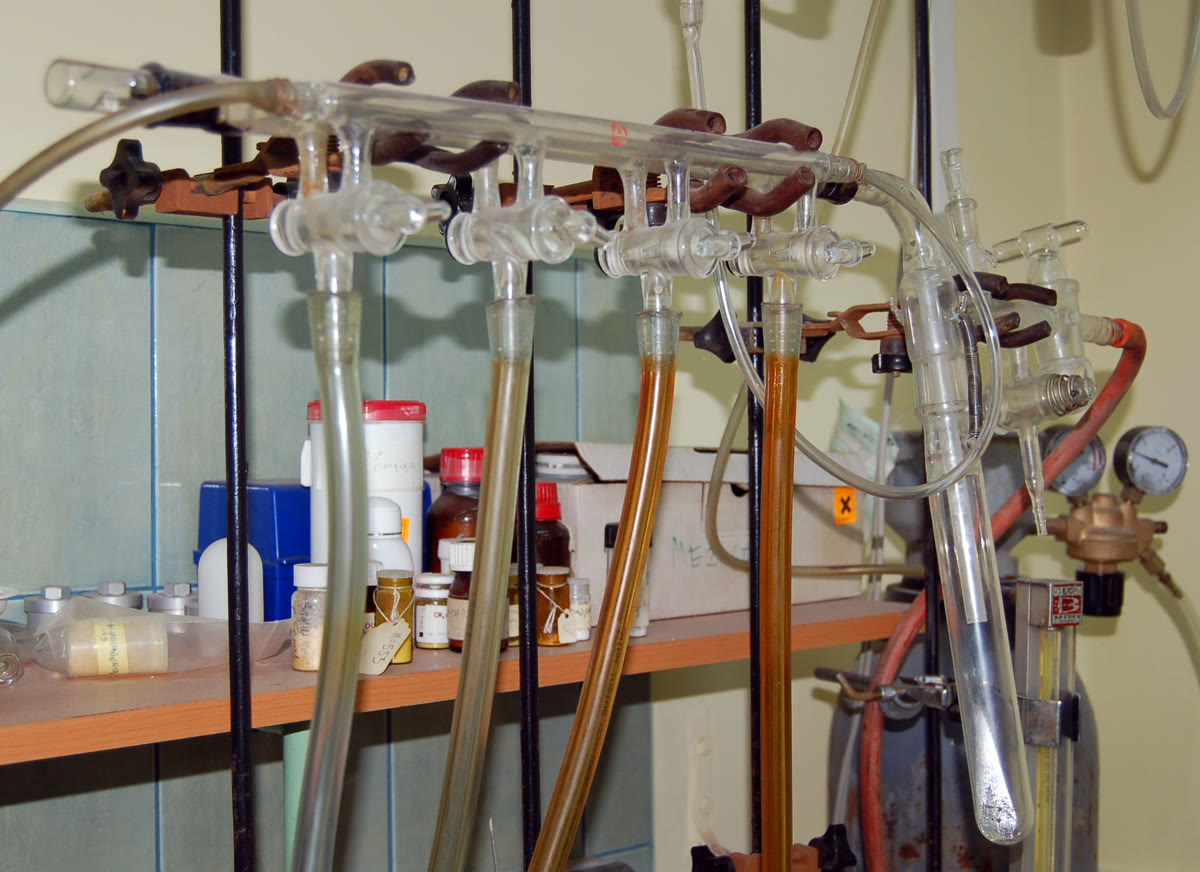
\includegraphics[width=0.46\linewidth]{images/book4/schlenk-line.jpg}

{\small Une \omterm{def:b3:lab-techniques-3:schlenk}{rampe de Schlenk} en service~: la rampe en verre et ses
robinets, les tuyaux vers les ballons, et le détendeur de gaz.
Photographie~: Polimerek, CC BY-SA 3.0.}
\end{omfigure}

\section{Caractériser un nouveau composé}

\begin{method}[Caractériser un nouveau composé]\label{met:b3:lab-techniques-3:characterise}
\begin{enumerate}
  \item Pureté~: une seule tache en CCM dans deux éluants, un seul pic en
        HPLC ou en CPG, un point de fusion net~; \omterm{def:b3:lab-techniques-3:qnmr}{RMN quantitative} si une
        pureté massique est nécessaire.
  \item Formule~: HRMS à quelques ppm de la masse calculée, et le profil
        isotopique~; ou \omterm{def:b3:lab-techniques-3:elemental}{analyse élémentaire}.
  \item Structure~: RMN du $^1$H et du $^{13}$C, avec des expériences 2D pour les connexions
        (\cref{ch:b3:advanced-nmr}), IR pour les groupes fonctionnels~;
        structure par diffraction des rayons X sur monocristal quand des
        cristaux se forment (\cref{ch:b3:x-ray-diffraction}).
  \item Stéréochimie~: NOE, constantes de couplage, pouvoir rotatoire, ee
        par chromatographie chirale.
  \item Rapporter chaque donnée avec ses conditions, et les spectres dans
        les \omterm{def:b3:lab-techniques-3:literature}{informations complémentaires}.
\end{enumerate}
\end{method}

\begin{omfigure}
\begin{tikzpicture}[font=\scriptsize, >=Stealth,
  box/.style={draw, rounded corners, align=center, fill=omDef!8, inner sep=3pt, minimum height=8mm}]
  \node[box] (a) at (0,0) {nouveau composé\\ isolé};
  \node[box] (b) at (2.85,0) {pur~?\\ CCM, HPLC, F};
  \node[box] (c) at (5.85,0) {formule\\ HRMS, CHN};
  \node[box] (d) at (8.75,0) {structure\\ RMN (1D, 2D), IR};
  \node[box] (e) at (8.75,-1.6) {rayons X si cristaux,\\ stéréochimie};
  \node[box, fill=omMeth!12] (f) at (5.85,-1.6) {cohérent~?\\ rapporter\\ avec les données\\ brutes};
  \node[box, fill=omThm!10] (g) at (2.85,-1.6) {purifier de nouveau\\ (chromatographie,\\ cristallisation)};
  \draw[->, thick] (a) -- (b); \draw[->, thick] (b) -- node[above, inner sep=1pt] {oui} (c);
  \draw[->, thick] (c) -- (d); \draw[->, thick] (d) -- (e); \draw[->, thick] (e) -- (f);
  \draw[->, thick] (b) -- node[left] {non} (g); \draw[->, thick] (g.north west) to[bend left=30] (a.south);
\end{tikzpicture}

{\small Le déroulement de la caractérisation d'un nouveau composé~: d'abord
la pureté, puis la formule, puis la structure~; chaque affirmation repose
sur au moins deux méthodes indépendantes, et les \omterm{def:b3:lab-techniques-3:notebook}{données brutes}
accompagnent le rapport.}
\end{omfigure}

\begin{definition}[Analyse élémentaire]\label{def:b3:lab-techniques-3:elemental}
L'\emph{analyse élémentaire}\index{analyse elementaire@analyse élémentaire} (analyse par combustion)
détermine les pourcentages massiques de carbone, d'hydrogène, d'azote et
de soufre d'un échantillon en le brûlant dans le dioxygène et en mesurant
le dioxyde de carbone, l'eau, le diazote et le dioxyde de soufre formés.
\end{definition}

\begin{proposition}[Pourcentages massiques à partir d'une formule]\label{prop:b3:lab-techniques-3:mass-fractions}
Pour une formule $\mathrm{C}_a\mathrm{H}_b\mathrm{N}_c\dots$ de masse molaire $M$, le pourcentage massique de carbone vaut $100\,aA_r(\mathrm C)/M$, et de même
pour les autres éléments.
\end{proposition}

\begin{proof}
Une mole de composé, de masse $M$, contient $a$ moles d'atomes de carbone, de masse $aA_r(\mathrm C)$~;
le rapport, multiplié par 100, est le pourcentage massique.
\end{proof}

% ledger: ea:tolerance, hrms:tolerance
La plupart des revues de chimie exigent des valeurs trouvées de C, H et N à
moins de 0.4 point de pourcentage des valeurs calculées, ou une mesure
HRMS à quelques ppm près (5 ppm pour certaines), comme preuve de la
composition. Une vaste étude interlaboratoires a montré que même des
échantillons purs manquent étonnamment souvent le critère de 0.4, ce qui
rappelle qu'un critère n'est pas une loi de la nature.

\begin{proposition}[Erreur en HRMS]\label{prop:b3:lab-techniques-3:ppm-error}
L'erreur d'une masse mesurée $m_{\mathrm{meas}}$ par rapport à la masse calculée $m_{\mathrm{calc}}$ vaut
$10^6(m_{\mathrm{meas}} - m_{\mathrm{calc}})/m_{\mathrm{calc}}$ ppm~; pour un ion, $m_{\mathrm{calc}}$ se calcule à partir des masses monoisotopiques moins (ou plus) la
masse des électrons retirés (ou ajoutés).
\end{proposition}

\begin{proof}[Par définition]
L'erreur en ppm est l'écart relatif exprimé en parties par million~; la
masse de l'ion diffère de celle de la formule neutre par les électrons, \qty{5.486e-4}{u} chacun, soit
quelques ppm pour des masses de quelques centaines.
\end{proof}

\begin{definition}[RMN quantitative]\label{def:b3:lab-techniques-3:qnmr}
La \emph{RMN quantitative}\index{RMN quantitative} (qNMR) détermine des
quantités ou des puretés à partir des intégrales des signaux, qui sont
proportionnelles au nombre de noyaux lorsque le spectre est enregistré
avec une relaxation complète entre les impulsions, par rapport à un étalon
interne de pureté connue pesé avec l'échantillon.
\end{definition}

\begin{proposition}[Pureté par qNMR]\label{prop:b3:lab-techniques-3:qnmr}
Pour un échantillon de masse $m_x$ pesé avec un étalon de masse $m_s$ et de pureté $P_s$, avec des signaux
d'intégrales $I_x$ et $I_s$ provenant de $N_x$ et $N_s$ protons,
\[
  P_x = \frac{I_x}{I_s}\,\frac{N_s}{N_x}\,\frac{M_x}{M_s}\,\frac{m_s}{m_x}\,P_s.
\]
\end{proposition}

\begin{proof}
Les intégrales des signaux sont proportionnelles aux nombres de protons~: $I_x/I_s = (N_xn_x)/(N_sn_s)$. Avec
$n_x = P_xm_x/M_x$ et $n_s = P_sm_s/M_s$, la résolution en $P_x$ donne la formule.
\end{proof}

\begin{omfigure}
\begin{tikzpicture}
\begin{axis}[width=0.8\linewidth, height=5.0cm, x dir=reverse, xmin=3.0, xmax=7.0, ymin=-0.05, ymax=1.15, clip=false,
  axis x line=bottom, axis y line=none, xlabel={$\delta$ / ppm}, tick label style={font=\scriptsize}, label style={font=\small}]
\addplot[color=omDef, thick] table[x=ppm, y=y] {figdata/out/bachelor-3-qnmr.dat};
\node[font=\scriptsize, anchor=south] at (axis cs:6.09,0.33) {étalon, ArH (3 H)};
\node[font=\scriptsize, anchor=east] at (axis cs:4.20,0.98) {ferrocène (10 H)};
\node[font=\scriptsize, anchor=west, align=left] at (axis cs:3.72,0.70) {étalon,\\ $\ce{OCH3}$ (9 H)};
\end{axis}
\end{tikzpicture}

{\small Spectre de proton synthétique d'un échantillon de ferrocène pesé
avec du 1,3,5-triméthoxybenzène comme étalon interne (modèle~: 20.0 mg
d'échantillon pur à 98.0\,\%, 15.0 mg d'étalon). Les intégrales sont
proportionnelles au nombre de protons multiplié par la quantité de chaque
composé~; le rapport du singulet du ferrocène au singulet aromatique de
l'étalon donne la pureté.}
\end{omfigure}

\section{Statistique d'un résultat de recherche}

\begin{definition}[Tests de signification]\label{def:b3:lab-techniques-3:tests}
Un \emph{test de signification}\index{test de signification} décide si des
données sont compatibles avec une \emph{hypothèse nulle}\index{hypothese nulle@hypothèse nulle}, en général
l'absence de différence ou d'effet, pour un niveau choisi de risque de la
rejeter à tort (souvent 5\,\%).
\end{definition}

\begin{theorem}[Test $t$ sur deux échantillons]\label{thm:b3:lab-techniques-3:t-test}
Pour deux séries de $n_1$ et $n_2$ mesures indépendantes tirées de lois normales
de même écart type, de moyennes $\bar x_1$, $\bar x_2$ et d'écart type
commun $s_p$, la statistique $t = (\bar x_1 - \bar x_2)/(s_p\sqrt{1/n_1 + 1/n_2})$ suit la loi de Student à
$n_1 + n_2 - 2$ degrés de liberté lorsque les deux moyennes vraies sont égales. \admitted
\end{theorem}

\begin{proposition}[Test $F$]\label{prop:b3:lab-techniques-3:f-test}
Sous les mêmes hypothèses, le rapport $F = s_1^2/s_2^2$ de deux variances d'échantillon suit
la loi de Fisher à $(n_1 - 1, n_2 - 1)$ degrés de liberté lorsque les variances vraies sont égales.
\admitted
\end{proposition}

\begin{method}[Un nouveau rendement est-il meilleur~?]\label{met:b3:lab-techniques-3:compare-means}
\begin{enumerate}
  \item Répéter les deux modes opératoires plusieurs fois dans les mêmes
        conditions~; consigner chaque résultat.
  \item Comparer d'abord les dispersions (test $F$)~; si elles sont semblables, les regrouper~:
        $s_p^2 = [(n_1 - 1)s_1^2 + (n_2 - 1)s_2^2]/(n_1 + n_2 - 2)$.
  \item Calculer $t$ et comparer $|t|$ au coefficient de Student pour $n_1 + n_2 - 2$ degrés de
        liberté au niveau choisi.
  \item Plus grand~: la différence est significative. Plus petit~: les
        données n'en montrent pas, ce qui ne prouve pas qu'il n'y en a
        aucune.
\end{enumerate}
\end{method}

Une valeur suspecte n'est jamais supprimée parce qu'elle dérange. Les tests
de valeurs aberrantes la signalent, mais la décision repose sur le \omterm{def:b3:lab-techniques-3:notebook}{cahier
de laboratoire}~: une cause consignée (une erreur de pesée, un ballon
contaminé) justifie de la rejeter~; sans cause, on la garde, ou l'on
refait l'expérience.

\section{Le cahier de laboratoire, les données de recherche et la littérature}

\begin{definition}[Cahier de laboratoire et données brutes]\label{def:b3:lab-techniques-3:notebook}
Le \emph{cahier de laboratoire}\index{cahier de laboratoire} est le relevé
daté, continu et non modifié des expériences réalisées, telles qu'elles
ont été réalisées. Les \emph{données brutes}\index{donnees brutes@données brutes} sont les
enregistrements originaux des mesures (fichiers des instruments, tickets
de pesée, spectres) avant tout traitement.
\end{definition}

\begin{method}[Rédiger une entrée du cahier de laboratoire]\label{met:b3:lab-techniques-3:notebook}
\begin{enumerate}
  \item Date, titre, objectif, et renvoi à l'expérience apparentée
        précédente.
  \item Le schéma réactionnel avec les quantités (masses, volumes, moles,
        équivalents), l'origine et les lots des réactifs, et l'\omterm{def:b3:lab-techniques-3:assessment}{évaluation
        des risques}.
  \item Ce qui a été fait et observé, dans l'ordre et sur le moment, y
        compris ce qui a mal tourné~; ne jamais effacer, barrer de sorte que
        l'original reste lisible.
  \item Résultats~: rendements, noms des fichiers de \omterm{def:b3:lab-techniques-3:notebook}{données brutes}, et une
        conclusion~; signer.
\end{enumerate}
\end{method}

\begin{definition}[Données FAIR]\label{def:b3:lab-techniques-3:fair}
% ledger: fair:year
Les \emph{données FAIR}\index{donnees FAIR@données FAIR} sont des données de recherche faciles
à trouver, accessibles, interopérables et réutilisables (en anglais
\textit{Findable, Accessible, Interoperable, Reusable})~: décrites par des
métadonnées riches et un identifiant pérenne, récupérables par des
protocoles standard, dans des formats ouverts, avec une licence et une
provenance claires.
\end{definition}

\begin{definition}[Intégrité scientifique]\label{def:b3:lab-techniques-3:integrity}
L'\emph{intégrité scientifique}\index{integrite scientifique@intégrité scientifique} est la conduite et la
communication honnêtes et transparentes de la recherche. Ses manquements
les plus graves sont la \emph{fabrication}\index{fabrication} (inventer des données), la \emph{falsification}\index{falsification}
(altérer des données, des images ou des modes opératoires) et le \emph{plagiat}\index{plagiat}
(présenter le travail d'autrui comme le sien).
\end{definition}

\begin{definition}[La littérature]\label{def:b3:lab-techniques-3:literature}
La \emph{littérature primaire}\index{litterature primaire@littérature primaire} rapporte des
recherches originales (articles, brevets, thèses)~; la \emph{littérature secondaire}\index{litterature secondaire@littérature secondaire} les passe en revue et les organise (articles de
synthèse, ouvrages de référence, bases de données), et les manuels forment
une couche tertiaire. L'\emph{évaluation par les pairs}\index{evaluation par les pairs@évaluation par les pairs} est l'examen d'un manuscrit par des
experts indépendants avant publication. Les \emph{informations complémentaires}\index{informations complementaires@informations complémentaires}
d'un article contiennent les détails expérimentaux et les données
nécessaires pour reproduire et vérifier le travail.
\end{definition}

\begin{method}[Lire un mode opératoire publié]\label{met:b3:lab-techniques-3:read-paper}
\begin{enumerate}
  \item Lire la partie expérimentale et les \omterm{def:b3:lab-techniques-3:literature}{informations complémentaires},
        pas seulement le résumé et le schéma.
  \item Vérifier l'échelle, les concentrations, les températures, les
        durées et le traitement~; noter ce qui manque.
  \item Vérifier la caractérisation des produits à l'aide de la méthode
        ci-dessus.
  \item Chercher les articles ultérieurs qui ont utilisé ou corrigé le mode
        opératoire~; le réaliser d'abord à petite échelle.
\end{enumerate}
\end{method}

Les bases de données de structures et de réactions indexent la \omterm{def:b3:lab-techniques-3:literature}{littérature
primaire} par composé et par transformation, et s'interrogent en dessinant
une structure ou une réaction plutôt qu'avec des mots.

\section{Évaluation des risques d'un nouveau mode opératoire}

\begin{definition}[Évaluation des risques]\label{def:b3:lab-techniques-3:assessment}
L'\emph{évaluation des risques}\index{evaluation des risques@évaluation des risques} d'un mode opératoire identifie
ses dangers, estime la probabilité et la gravité des dommages dans les
conditions prévues, et fixe les mesures qui ramènent le risque à un niveau
acceptable. La \emph{hiérarchie des mesures de prévention}\index{hierarchie des mesures de prevention@hiérarchie des mesures de prévention} les classe de la plus à la
moins efficace~: élimination, substitution, protection collective,
mesures organisationnelles, équipements de protection individuelle.
\end{definition}

\begin{omfigure}
\begin{tikzpicture}[font=\scriptsize]
  \foreach \i/\lab/\col in {0/élimination~: supprimer le danger/omMeth!40, 1/substitution~: un réactif moins dangereux/omMeth!28, 2/protection collective~: hotte{,} boîte à gants{,} écrans/omDef!22, 3/organisation~: modes opératoires{,} formation/omProp!22, 4/équipements de protection individuelle/omThm!22} {
    \pgfmathsetmacro\w{5.4-0.95*\i}
    \fill[\col] ({-\w/2},{-0.75*\i}) -- ({\w/2},{-0.75*\i}) -- ({\w/2-0.475},{-0.75*\i-0.7}) -- ({-\w/2+0.475},{-0.75*\i-0.7}) -- cycle;
    \node[anchor=west] at (3.0,{-0.75*\i-0.35}) {\lab};
    \draw[black!30] ({\w/2-0.2},{-0.75*\i-0.35}) -- (2.95,{-0.75*\i-0.35});
  }
  \node[anchor=east, align=right] at (-2.9,-0.35) {plus\\ efficace};
  \node[anchor=east, align=right] at (-2.9,-3.35) {moins\\ efficace};
  \draw[->, black!50] (-3.3,-0.85) -- (-3.3,-2.85);
\end{tikzpicture}

{\small La \omterm{def:b3:lab-techniques-3:assessment}{hiérarchie des mesures de prévention}, en pyramide inversée~:
supprimer ou remplacer le danger protège tout le monde, toujours~; un
équipement de protection ne protège que celui qui le porte, et seulement
s'il est porté et intact.}
\end{omfigure}

\begin{definition}[Composés peroxydables]\label{def:b3:lab-techniques-3:peroxide}
Un \emph{composé peroxydable}\index{compose peroxydable@composé peroxydable} est un composé, comme
l'éther diéthylique, le tétrahydrofurane ou le 1,4-dioxane, qui forme
lentement des peroxydes explosifs au contact de l'air pendant son
stockage, surtout après ouverture et à la lumière.
\end{definition}

\begin{method}[Évaluer les risques d'un nouveau mode opératoire]\label{met:b3:lab-techniques-3:risk-assessment}
\begin{enumerate}
  \item Lister chaque substance (réactifs, solvants, produits,
        sous-produits, gaz dégagés) avec ses dangers d'après la fiche de
        données de sécurité.
  \item Lister les opérations et leurs conditions (chauffage, pression,
        échelle, désactivation, déchets)~; estimer la chaleur dégagée et
        l'élévation adiabatique de température avant tout changement
        d'échelle.
  \item Pour chaque danger, choisir les mesures en descendant la
        hiérarchie~; prévoir la réponse aux situations d'urgence
        (déversement, incendie, exposition) et la filière des déchets.
  \item La mettre par écrit, la faire vérifier, et la réexaminer après la
        première mise en œuvre.
\end{enumerate}
\end{method}

\begin{safety}{\ghs[0.62cm]{GHS02}\ghs[0.62cm]{GHS05}\ghs[0.62cm]{GHS07}\ghs[0.62cm]{GHS08}}
% ledger: ghs4:BuLi, ghs4:Et2O, ghs4:THF
Solutions de butyllithium~: pyrophoriques, réagissent violemment avec
l'eau en libérant un gaz inflammable, provoquent de graves brûlures~;
manipulées uniquement sous gaz inerte, avec un seau de sable sec à portée
de main et sans eau à proximité. L'hydrure de sodium libère de même du
dihydrogène au contact de l'eau et de l'humidité, et s'utilise en
dispersion dans l'huile. L'éther diéthylique et le THF sont très
inflammables et \omterm{def:b3:lab-techniques-3:peroxide}{peroxydables}~: ils sont datés à l'ouverture, testés pour
les peroxydes avant toute distillation ou évaporation, et éliminés selon un
calendrier.
\end{safety}

\begin{history}[La verrerie de Schlenk]
Wilhelm Schlenk, qui étudiait les composés organoalcalins et les radicaux
dans les années 1910, conçut les ballons et les techniques qui lui
permirent de les manipuler à l'abri de l'air~; la rampe et le tube portent
toujours son nom. Les premières \omterm{def:b3:lab-techniques-3:schlenk}{boîtes à gants} furent construites dans les
années 1940 pour les matières radioactives, et bientôt adoptées par les
chimistes travaillant sur des \omterm{def:b3:lab-techniques-3:air-sensitive}{composés sensibles à l'air}.
\end{history}

\section{Exercices}

\begin{exercise}[$\star$]\label{exo:b3:lab-techniques-3:1}
Un ballon est vidé jusqu'à \qty{0.50}{mbar} et rempli d'argon jusqu'à \qty{1013}{mbar}, trois fois. Quelle fraction de
l'air initial reste-t-il, en théorie~? Qu'est-ce qui limite réellement le
résultat~?
\end{exercise}

\begin{exercise}[$\star$]\label{exo:b3:lab-techniques-3:2}
Une solution de butyllithium a un titre de \qty{1.48}{mol/L}. Quel volume faut-il transférer pour apporter
\qty{20.0}{mmol}~?
\end{exercise}

\begin{exercise}[$\star$]\label{exo:b3:lab-techniques-3:3}
% ledger: mass:C12, mass:H1, mass:Fe56, const4:me.u, hrms:tolerance
Calculer la masse exacte du cation radical du ferrocène $\ce{C10H10Fe+}$ à partir des masses monoisotopiques
($^{12}$C 12 exactement, $^1$H 1.00782503, $^{56}$Fe 55.93493633, électron \qty{5.486e-4}{u}), et l'erreur d'une valeur mesurée de
186.0129, en ppm.
\end{exercise}

\begin{exercise}[$\star$]\label{exo:b3:lab-techniques-3:4}
Classer en \omterm{def:b3:lab-techniques-3:literature}{littérature primaire}, secondaire ou tertiaire~: un article de
synthèse, un article de périodique rapportant une nouvelle synthèse, un brevet,
un recueil de constantes physiques, une thèse, un manuel.
\end{exercise}

\begin{exercise}[$\star\star$]\label{exo:b3:lab-techniques-3:5}
% ledger: ea:tolerance
Calculer les pourcentages massiques de C, H et N de la caféine, $\ce{C8H10N4O2}$, et dire si les valeurs
trouvées C 49.31, H 5.22, N 28.71\,\% satisfont au critère usuel de 0.4 point.
\end{exercise}

\begin{exercise}[$\star\star$]\label{exo:b3:lab-techniques-3:6}
Un échantillon de \qty{170.0}{mg} d'acide diphénylacétique ($\ce{C14H12O2}$) exige \qty{0.54}{mL} d'une solution de butyllithium pour atteindre
le virage au jaune. Calculer le titre.
\end{exercise}

\begin{exercise}[$\star\star$]\label{exo:b3:lab-techniques-3:7}
Un ancien mode opératoire a donné des rendements de 72, 75, 71, 74 et
73\,\%~; un mode modifié, 76, 78, 75, 77 et 79\,\%. Avec un coefficient de
Student de 2.31 pour 8 degrés de liberté à 95\,\% (données de l'exercice),
l'amélioration est-elle significative~?
\end{exercise}

\begin{exercise}[$\star\star$]\label{exo:b3:lab-techniques-3:8}
Deux méthodes donnent six résultats chacune, avec des écarts types de 0.80
et 0.30 (mêmes unités). Avec une valeur critique de $F$ de 5.05 pour (5, 5) degrés de liberté à 95\,\% (données de
l'exercice), leurs fidélités diffèrent-elles~?
\end{exercise}

\begin{exercise}[$\star\star$]\label{exo:b3:lab-techniques-3:9}
Proposer un plan de stockage et de contrôle pour les flacons de THF et
d'éther diéthylique d'un laboratoire.
\end{exercise}

\begin{exercise}[$\star\star\star$]\label{exo:b3:lab-techniques-3:10}
Un étudiant prévoit de déprotoner un alcool par l'hydrure de sodium dans
le DMF à 60 °C à l'échelle de 50 g. Identifier les dangers (y compris les
dangers thermiques de ce solvant avec la base) et choisir les mesures en
descendant la hiérarchie.
\end{exercise}

\begin{exercise}[$\star\star\star$]\label{exo:b3:lab-techniques-3:11}
Propager les incertitudes-types relatives de $I_x$, $I_s$ (0.50\,\% chacune), $m_x$ et $m_s$ (\qty{0.010}{mg} sur 20.0
et 15.0 mg) et $P_s$ (0.10\,\%) dans la formule de la qNMR, et donner l'incertitude relative de $P_x$.
Quel terme domine~?
\end{exercise}

\begin{exercise}[$\star\star\star$]\label{exo:b3:lab-techniques-3:12}
Cinq titrages donnent 81.2, 82.0, 80.6, 81.5 et 89.0 (en mL). Un test de
Dixon donne
$Q = 0.83$ pour une valeur critique de 0.71 (données de l'exercice). Faut-il rejeter la dernière
valeur~? Expliquer ce qu'il faudrait vérifier d'abord.
\end{exercise}

\section{Problème~: du ballon à la publication}

\begin{problem}[{Problème du week-end --- du ballon à la publication, un
nouveau composé sensible à l'air~: la synthèse du ferrocène sous diazote,
sa caractérisation, sa pureté par RMN quantitative, et l'évaluation des
risques du mode opératoire}]
\label{pb:b3:lab-techniques-3:1}
% ledger: aw:C, aw:H, aw:Fe, aw:Cl, aw:O, mass:C12, mass:H1, mass:Fe56, const4:me.u, ghs4:ferrocene
Données du problème. Le chlorure de fer(II) anhydre (5.00 g) réagit avec le
cyclopentadiénure de sodium (deux équivalents, préparé à partir de
cyclopentadiène et d'hydrure de sodium dans le
THF) sous diazote~; on isole 5.86 g de ferrocène orange, $\ce{Fe(C5H5)2}$. Les ballons sont
purgés par trois cycles jusqu'à \qty{0.10}{mbar} à partir de \qty{1000}{mbar}. La HRMS donne $m/z$ 186.0129 pour $\ce{M+}$~; l'\omterm{def:b3:lab-techniques-3:elemental}{analyse
élémentaire}, C 64.41, H 5.47\,\%. Dans $\ce{CDCl3}$, le ferrocène donne un singulet à 4.16 ppm (10 H). Pour la qNMR,
20.0 mg de l'échantillon et 15.0 mg de 1,3,5-triméthoxybenzène (pureté 99.9\,\%, singulet
aromatique à 6.09 ppm, 3 H) donnent $I_x/I_s = 3.942$, avec des incertitudes-types relatives de 0.50\,\% pour chaque
intégrale, de \qty{0.010}{mg} pour chaque masse et de 0.10\,\% pour $P_s$.

\medskip\noindent\textbf{Partie I --- La synthèse sous diazote.}
\begin{enumerate}
  \item Écrire l'équation de la synthèse.
  \item Pourquoi faut-il mener la réaction à l'abri de l'air~?
  \item Calculer la masse théorique de ferrocène et le rendement.
  \item Calculer la fraction d'air qui reste après les trois cycles de
        purge.
  \item Comment obtient-on le cyclopentadiène à partir de son dimère, et
        pourquoi faut-il l'utiliser aussitôt~?
  \item Pourquoi l'hydrure de sodium est-il ajouté par portions~?
\end{enumerate}

\medskip\noindent\textbf{Partie II --- La caractérisation.}
\begin{enumerate}[resume]
  \item Calculer la masse exacte de $\ce{M+}$ et l'erreur de la mesure en ppm.
  \item Calculer les pourcentages massiques de C et de H et les comparer à
        l'analyse.
  \item Pourquoi le ferrocène ne présente-t-il qu'un seul signal en RMN du $^1$H~?
  \item Que montrerait la RMN du $^{13}$C~?
  \item Quelle autre méthode prouverait la structure sandwich~?
  \item Le ferrocène lui-même est-il sensible à l'air une fois formé~?
        Comparer à ses précurseurs.
\end{enumerate}

\medskip\noindent\textbf{Partie III --- Pureté par qNMR.}
\begin{enumerate}[resume]
  \item Pourquoi choisir ici le 1,3,5-triméthoxybenzène comme étalon~?
  \item Que doit garantir l'acquisition RMN pour que les intégrales soient
        quantitatives~?
  \item Calculer les masses molaires du ferrocène et de l'étalon.
  \item Calculer la pureté de l'échantillon.
  \item Calculer son incertitude-type relative et absolue.
  \item L'\omterm{def:b3:lab-techniques-3:elemental}{analyse élémentaire} est-elle cohérente avec cette pureté~?
\end{enumerate}

\medskip\noindent\textbf{Partie IV --- Les risques et une dernière mesure.}
\begin{enumerate}[resume]
  \item Lister les dangers du mode opératoire.
  \item Choisir les mesures pour l'hydrure de sodium et pour le THF.
  \item Comment faut-il détruire l'excès d'hydrure de sodium à la fin~?
  \item Que montre un \omterm{def:b3:electrode-kinetics:cv}{voltampérogramme} cyclique du ferrocène, et pourquoi
        utilise-t-on le ferrocène comme référence en électrochimie~?
  \item Que doivent contenir l'entrée du \omterm{def:b3:lab-techniques-3:notebook}{cahier de laboratoire} et les
        \omterm{def:b3:lab-techniques-3:literature}{informations complémentaires}~?
  \item Pourquoi faut-il archiver les spectres bruts dans un format ouvert~?
  \item Énoncer le résultat~: la pureté qNMR de l'échantillon de ferrocène,
        avec son incertitude-type.
\end{enumerate}
\end{problem}
